\documentclass[12pt]{article}
\usepackage{amsmath}
\usepackage[margin = 1in]{geometry}
\usepackage{graphicx}
\usepackage{booktabs}
\usepackage{hyperref}
\usepackage{cleveref}
\hypersetup{colorlinks = true, linkcolor = blue, citecolor=blue, urlcolor = blue}
\usepackage{natbib}
\usepackage{natbib}
\usepackage{float}
\usepackage{pdfpages}




\usepackage{lipsum}

\usepackage[colorlinks=true, citecolor=blue]{hyperref}



\title{UCSAS 2024 USOPC Data Challenge}
\author{Kathleen Houlihan\\
  Department of Statistics\\
  University of Connecticut
}

\begin{document}
\maketitle

\begin{abstract}

 At the Summer Olympics in Paris in 2024, ninety-six men and ninety-six women 
 from around the world will compete on various apparatus. Twelve teams of five athletes will be 
 featured in the team events for both men's and women's events. In terms of events, women
 will compete on four apparatus while men will compete on six apparatus. This paper along 
 with my senior honors thesis will focus on the completion of the UCSAS 2024 USOPC Data Challenge. 
 The UCSAS 2024 USOPC Data Challenge tasks individuals with developing an analytics model that
 can be used to identify and compare the expected medal count for the United States male and 
 female artistic gymnasts at the 2024 Summer Olympics in Paris. At the Olympics there are 8 
 medal events for men consisting of team all-around, individual all-around, floor exercise, 
 pommel horse, still rings, vault, parallel bars, and high bar and 6 medal events for the women 
 consisting of team all-around, individual all-around, vault, uneven bars, balance beam, and 
 floor exercise. In this paper, I will identify which five female artistic gymnasts 
 are best suited to be sent to the Paris 2024 Olympics on behalf of the United States in order 
 to maximize the expected medal count. In my full honors thesis, I will use the methods outlined in this 
 paper to identify which five female and male athletes are best suited to be sent to the Paris 2024 
 Olympics on behalf of the United States and I will also calculate the expected medal count.

\end{abstract}

\section{Introduction}
\label{sec:intro}

The Summer and Winter Olympics are held every four years, traditionally in a unique country and city.
The importance of the Olympics cannot be understated as the games are a symbol of peaceful global 
interaction and give people hope that a better world is possible. For decades, gymnastics  
has been the most watched sport in the Summer Olympics and the United States has been known for bringing gold 
medal-winning gymnasts to compete. In the 2020 Summer Olympics games in Tokyo, the United States 
female artistic gymnastics team took home the gold medal in the Women's All Around, a bronze medal 
in the Women's Balance Beam, a gold medal in the Women's Floor Exercise, a silver medal for the Women's
Team, a bronze medal in the Women's Uneven Bars, and a silver medal in the Women's Vault. 
Noting that the United States was the only country to have a team medal in all six women's artistic gymnastics 
categories, the likely hood of the United States bringing female athletes that will medal in the 2024 
Paris Olympics is very probable. However, in the 2020 Summer Olympic games in Tokyo, the United States 
male artistic gymnastics team did not medal at all. This data challenge not only tasks individuals 
with predicting the expected medal count, but also predicting which athletes the United States will 
and should select to bring to the Paris 2024 Summer Olympics in order to maximize the number of medals 
the Unites States teams win. 
\\
The challenge of selecting a team of five athletes to represnet the United States at the Paris 2024 Olympics is 
complicated by the layout of the Olympic artictic gymnastics competition. While five athletes compete at the 
Olympic games, all five athletes do not compete on all four female gymnastic apparatuses. For the team all-around 
medal, four athletes compete on all four apparatuses in the qualifying round and the sum of the top three of four scores 
on each apparatus is calculated to determine if the team advances to the team all-around finals. If a team 
is among the top eight teams to advance, scores from the qualifying round are discared and three athletes from each 
team compete on all four apparatuses again and all three scores on each apparatus are summed and compared to that 
of the other teams. In order to be eligible to compete for the individual all-around medal, an athlete must be 
one of the four athletes that competed on all apparatuses in the qualifying round. If an athlete is among the top 
24 athletes to advance to the individual all-around final based on the sum of their scores on each apparatus, 
scores from the qualifying round are discarded and each athlete competes on all four apparatuses again. Despite 
the fact that four athletes compete on all apparatuses in the qualifying round, only two athletes from each country 
are allowed to advance to the individual all-around finals. Additionally, the top eight athletes on each apparatus 
during the qualifying round are able to advance to the finals for that apparatus. Similar to the individual all-around, 
finals, a maximum of two athletes per country can attend the finals for each apparatus. Using this information, I am 
tasked with determining which combination of five female athletes will maximize the number of medals the United 
States female team wins.

\\

The rest of this paper is organized as follows. First, I will discuss the literature that is relevant to 
my research in Section~\ref{sec:lit}. Next, I will identify the data that is available in order to complete 
this project in Section~\ref{sec:data}. Then, I will discuss my 
analytical methods to determine the atheltes that should be sent to the Olympics from the United States 
in Section~\ref{sec:meth}. Later, I will present the results of my 
methods in Section~\ref{sec:res}. Lastly, I will discuss the meaning of my results, some challenges, 
and some limitations of this project in Section~\ref{sec:dis}.

\section{Literature Review}
\label{sec:lit}

There is literature

\section{Data}
\label{sec:data}

This year, the University of Connecticut Sports Analytic Symposium (UCSAS) and the United States 
Olympic and Paralympic Committee has released a data challenge focused on identifying a group of 
five athletes who will enable the United States Men's and Women's Artistic Gymnastics teams to 
maximize earned medals at the Paris 2024 Summer Olympics. To predict which of the United States 
athletes are most likely to medal on the various apparatuses, I will be using the cleaned data that 
is provided in the UCSAS data challenge that includes data from major domestic and international 
gymnastic competitions from 2022 and 2023. The cleaned data provides the last name, first name, gender, 
country, date, competition, round, location, apparatus, rank, difficulty score, execution score, penalty, 
and overall score of various potential Olympic athletes at various competitions. This data is available, 
public, and already cleaned to be easily loaded into R studio where the majority of the computations 
required of this project will be completed. 
\\
The UCSAS data challenge also provides data from major domestic
and international gymnastic competions from 2017 to 2021 which must be kept separate from the more recent 2022 
and 2023 data due to the fact that the Code of Points scoring system is changed each Olympic cycle. Regardless 
of this fact, the primary data source for this paper will be the data from 2022 and 2023, as time, injuries, 
and other factors can have a large impact on the success of a gymnast, so the greatest predictor
of the Olympic outcomes in 2024 will be the most recent data.
\\
For the purposes of my research design, I limited the data I utilized to only include female United States
gymnasts. Furthermore, I processed the data to remove any scores of zero based on the assumption that these may 
be indicative of missing scores and that instances of these scores are rare. I further justified my decision 
to eliminate scores of zero for the purposes of knowing the true mean scores of each athlete on each 
apparatus for each successful attempt. Additionally, for some athletes and competitions, I found that the vault
apparatus was listed as "VT," "VT1," and "VT2." This discrepancy is due to the fact that athletes are permitted
two attempts on the vault apparatus. In an effort to interpret the data as accurately as possible and avoid having 
multiple statistics for one athlete on the same apparatus, I corrected this discrepancy by merging "VT," "VT1," and 
"VT2" to all be reported at "VT." Also, the data source is flawed as it alternates between reporting athlete names
in upper or lower case letters. In order to correct this, I converted all last names to lower case for consistency 
purposes. Lastly, the data source is inconsistent in the manner that it reports the first names of athletes as certain
athletes are listed using only their first name at some competitions and are listed using their first and middle names 
under the "first name" category for other competitions. In order to resolve this discrepancy, I manually verified that 
any athletes listed under two names were the same person and I further verified that there were no United States female 
athletes with the same last name so that all statistical computations could be completed through grouping by last 
name alone.

\section{Methods}
\label{sec:meth}

The most important task of the larger project involves determining which 5 athletes
should be brought to the 2024 Olympics in order to maximize success. For women, this means determining 
which five athletes stand the greatest chance of winning the gold medal for the women's individual all-around,
team all-around, Balance Beam, Floor Exercise, Uneven Bars, and Vault. 

In order to select the appropriate athletes, I first processed the data as described in Section~\ref{sec:data}.
Then, I calculated and examined the mean and standard deviations of each American female athlete's score 
on each apparatus. I also examined the number of observations for each athlete on each apparatus to familiarize 
myself with which athletes tend to compete at the most competitions and on which apparatuses. Then, I plotted 
the mean versus the standard deviation of the ten athletes with the highest mean scores on each apparatus. 
Using this visual, I created a parameter for each apparatus that uses both mean score and standard 
deviation to identify which athletes are best suited to be considered to compete on behalf of the United 
States on each apparatus. Using this parameter, I identified the "best" five athletes that compete on
each apparatus based on both their success, a high mean score, and their inconsistency, their standard deviation. 

Next, using only the athletes I identified as the "best" on each apparatus using the parameters, 
I calculated the sum of each athletes mean score for each apparatus and the sum of each athlete's standard 
deviation for each apparatus. Similarly to before, I plotted the mean score versus the standard deviation for 
these selected athletes. This plot is intended to represent
the United States' best candidates for earning a gold medal for the individual all-around component of the Olympics.

Then, using the sum of each selected athlete's mean score for each apparatus and the sum of each athlete's standard 
deviation for each apparatus which was previously calculated, I calculated the summed mean score and standard deviation sum 
of every combination of three athletes. Next, I plotted the summed mean score versus the standard deviation for the ten 
athlete combinations with the highest summed mean score. This plot is designed to identify the United States' best 
candidates for the all-around team finals.

Furthermore, using the sum of each selected athlete's mean score for each apparatus and the sum of each athlete's standard 
deviation for each apparatus which was previously calculated, I calculated the summed mean score and standard deviation sum 
of every combination of four athletes. Once again, I plotted the summed mean score versus the standard deviation for the ten 
athlete combinations with the highest summed mean score. This plot is designed to identify the United States' best 
candidates for the all-around team qualifying round.

Finally, in order to build a final team of five, we will manually examine all of the data in an effort to include in 
the final team the best three candidates for the team all-around, the best candidate for the fourth qualifying position, 
the best two candidates for the individual all-around, and the two athletes that are superior on each apparatus.


\section{Results}
\label{sec:res}

\begin{table}[tbp]
  \caption{The results of the mean and standard deviation calculations for the 10 athletes with the highest 
  mean scores on Balance Beam}
  \label{tab:tableBB}
\centering
\begin{tabular}[t]{lccllll}
  \toprule
  Apparatus & Last Name & Number of Observations & Mean Score & Standard Deviation\\
  \midrule
  BB & biles & 7 & 14.59986 & 0.2175794\\
  \midrule
  BB & mcclain & 3 14.50000 & 0.3605551\\
  \midrule
  BB & lee & 3 & 14.11667 & 0.4310839\\
  \midrule
  BB & frazier & 1 & 13.70000 & NA\\
  \midrule
  BB & blakely & 11 & 13.45591 & 0.6741748\\
  \midrule
  BB & sumanasekera & 7 & 13.43571 & 0.4867075\\
  \midrule
  BB & jones & 13 & 13.32169 & 0.7399390\\
  \midrule
  BB & wong & 8 & 13.16450 & 0.6798082\\
  \bottomrule
  \end{tabular}
  \end{table}

  \begin{table}[tbp]
    \caption{The results of the mean and standard deviation calculations for the 10 athletes with the highest 
    mean scores for Floor Exercise}
    \label{tab:tableFX}
\centering
\begin{tabular}[t]{lccllll}
   \toprule
  Apparatus & Last Name & Number of Observations & Mean Score & Standard Deviation\\
  \midrule
  FX & biles & 7 & 14.86643 & 0.3162630\\
  \midrule
  FX & lincoln & 6 & 14.00550 & 0.2753570\\
  \midrule
  FX & carey & 8 & 13.80188 & 0.3885270\\
  \midrule
  FX & chiles & 11 & 13.72873 & 0.3440930\\
  \midrule
  FX & jones & 14 & 13.70464 & 0.4150903\\
  \midrule
  FX & mcclain & 3 & 13.63333 & 0.4193249\\
  \midrule
  FX & dicello & 8 & 13.62487 & 0.2176225\\
  \midrule
  FX & roberson & 15 & 13.50773 & 0.5285517\\
  \midrule
  FX & frazier & 1 & 13.50000 & NA\\
  \midrule
  FX & wong & 6 & 13.46933 & 0.3093261\\
  \bottomrule
\bottomrule
  \end{tabular}
  \end{table} 

\begin{table}[tbp]
  \caption{The results of the mean and standard deviation calculations for the 10 athletes with the highest 
  mean scores on Uneven Bars}
  \label{tab:tableUB}
\centering
\begin{tabular}[t]{lccllll}
 \toprule
  Apparatus & Last Name & Number of Observations & Mean Score & Standard Deviation\\
  \midrule
  UB & jones & 15 & 14.50973 & 0.4934615\\
  \midrule
  UB & biles & 7 & 14.25700 & 0.1782797\\
  \midrule
  UB & miller & 9 & 14.00722 & 1.2597386\\
  \midrule
  UB & wong & 8 & 13.81025 & 0.4417128\\
  \midrule
  UB & blakely & 10 & 13.80650 & 0.6365863\\
  \midrule
  UB & matthews & 11 & 13.74245 & 0.4847538\\
  \midrule
  UB & chiles & 12 & 13.65967 & 0.6418676\\
  \midrule
  UB & walker & 1 & 13.55000 & NA\\
  \midrule
  UB & greaves & 2 & 13.52500 & 0.1060660\\
  \midrule
  UB & zhou & 4 & 13.50000 & 0.4415880\\
  \bottomrule
\bottomrule
  \end{tabular}
  \end{table}

 \begin{table}[tbp]
  \caption{The results of the mean and standard deviation calculations for the 10 athletes with the highest 
  mean scores on Vault}
  \label{tab:tableVT}
\centering
\begin{tabular}[t]{lccllll}
 \toprule
  Apparatus & Last Name & Number of Observations & Mean Score & Standard Deviation\\
  \midrule
  VT & biles & 9 & 14.98311 & 0.4120714\\
  \midrule
  VT & carey & 15 & 14.50213 & 0.2842868\\
  \midrule
  VT & jones & 11 & 14.28773 & 0.1783721\\
  \midrule
  VT & mcclain & 3 & 14.28333 & 0.1607275\\
  \midrule
  VT & richardson & 1 & 14.25000 & NA\\
  \midrule
  VT & chiles & 19 & 14.21826 & 0.2206148\\
  \midrule
  VT & blakely & 6 & 14.15000 & 0.2000000\\
  \midrule
  VT & sumanasekera & 6 & 14.11933 & 0.1056743\\
  \midrule
  VT & torry & 1 & 14.10000 & NA\\
  \midrule
  VT & dicello & 7 & 14.02843 & 0.2933677\\
   \bottomrule
\end{tabular}
\end{table}

\begin{figure}[tbp]
  \centering
  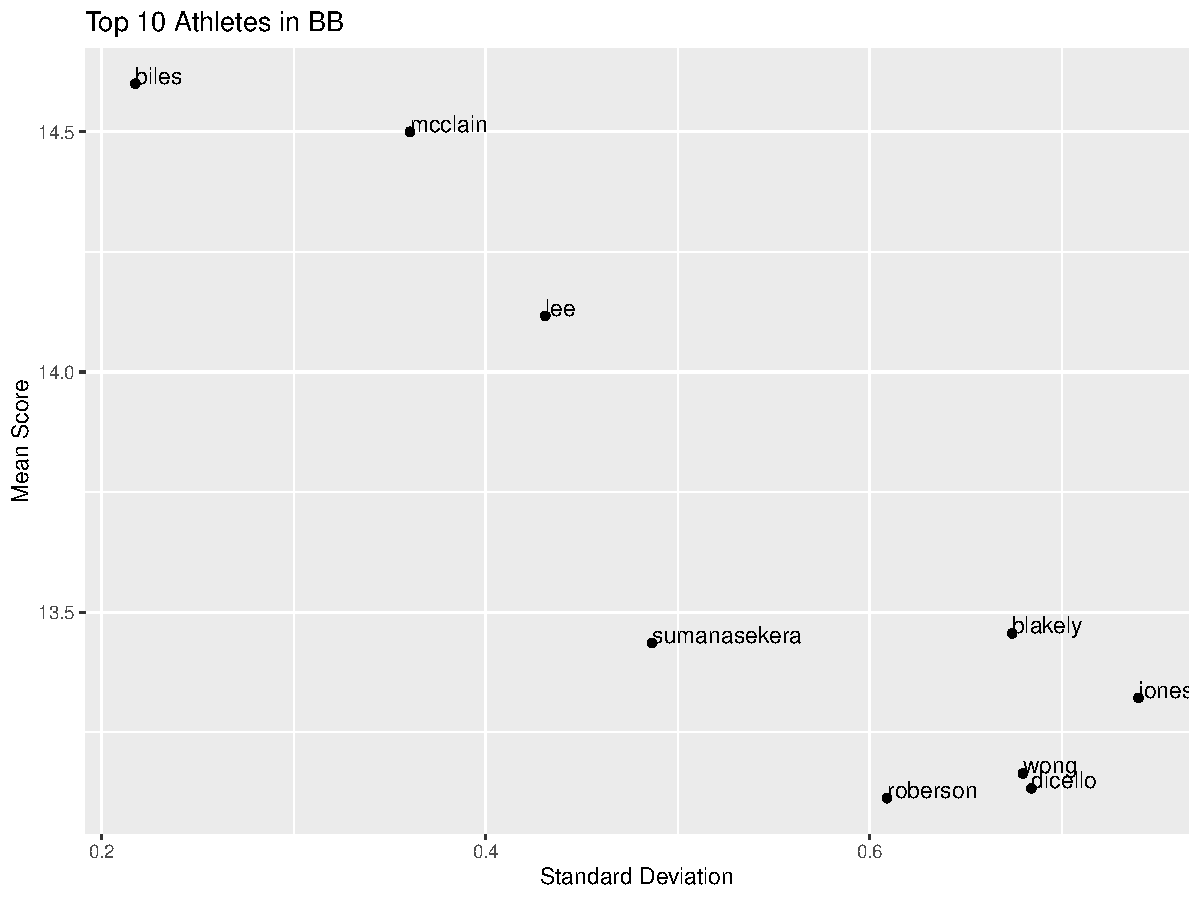
\includegraphics[scale=0.6]{Top10AthletesBB.pdf}
  \caption{Top 10 Candidates for the Olympic Balance Beam Apparatus}
  \label{fig:BB}
\end{figure}

\begin{figure}[tbp]
  \centering
  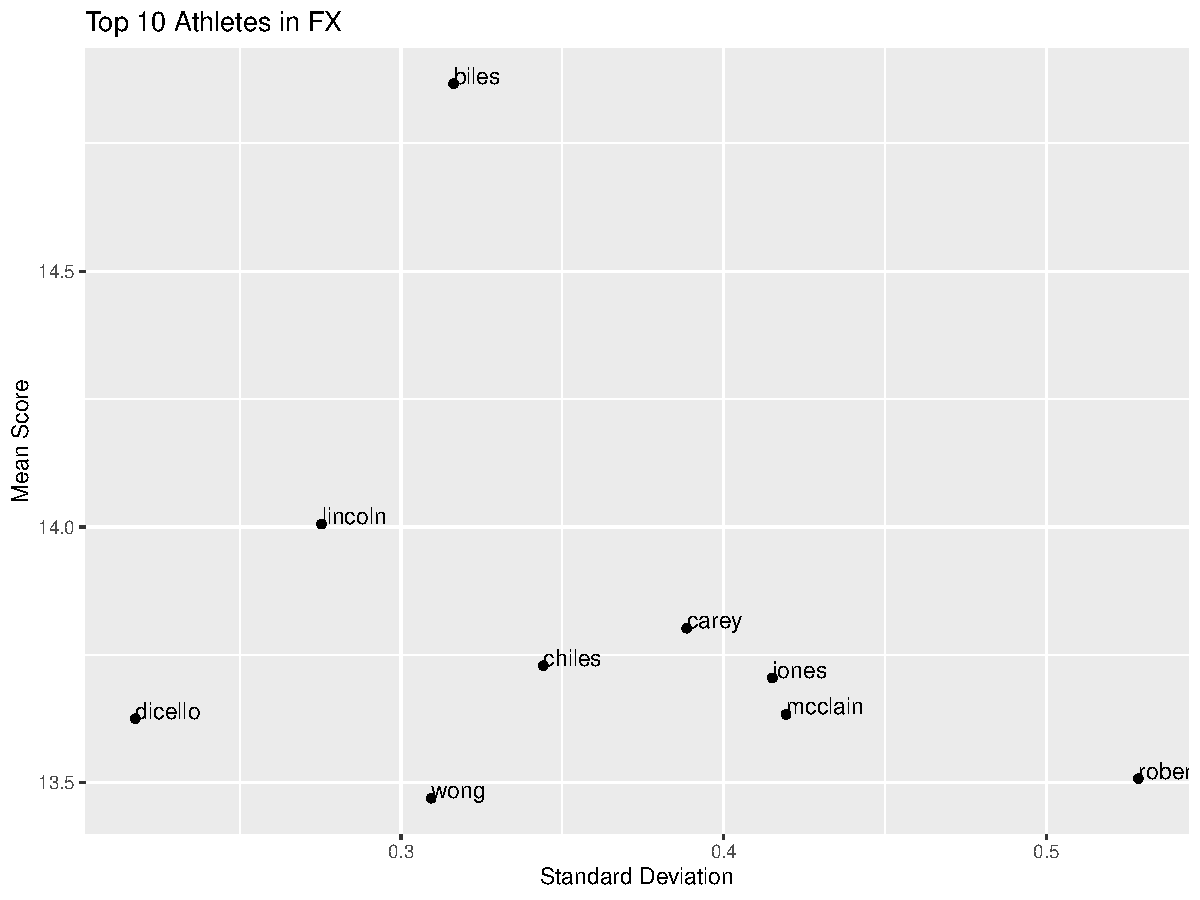
\includegraphics[scale=0.6]{Top10AthletesFX.pdf}
  \caption{Top 10 Candidates for the Olympic Floor Exercise Apparatus}
  \label{fig:FX}
\end{figure}

\begin{figure}[tbp]
  \centering
  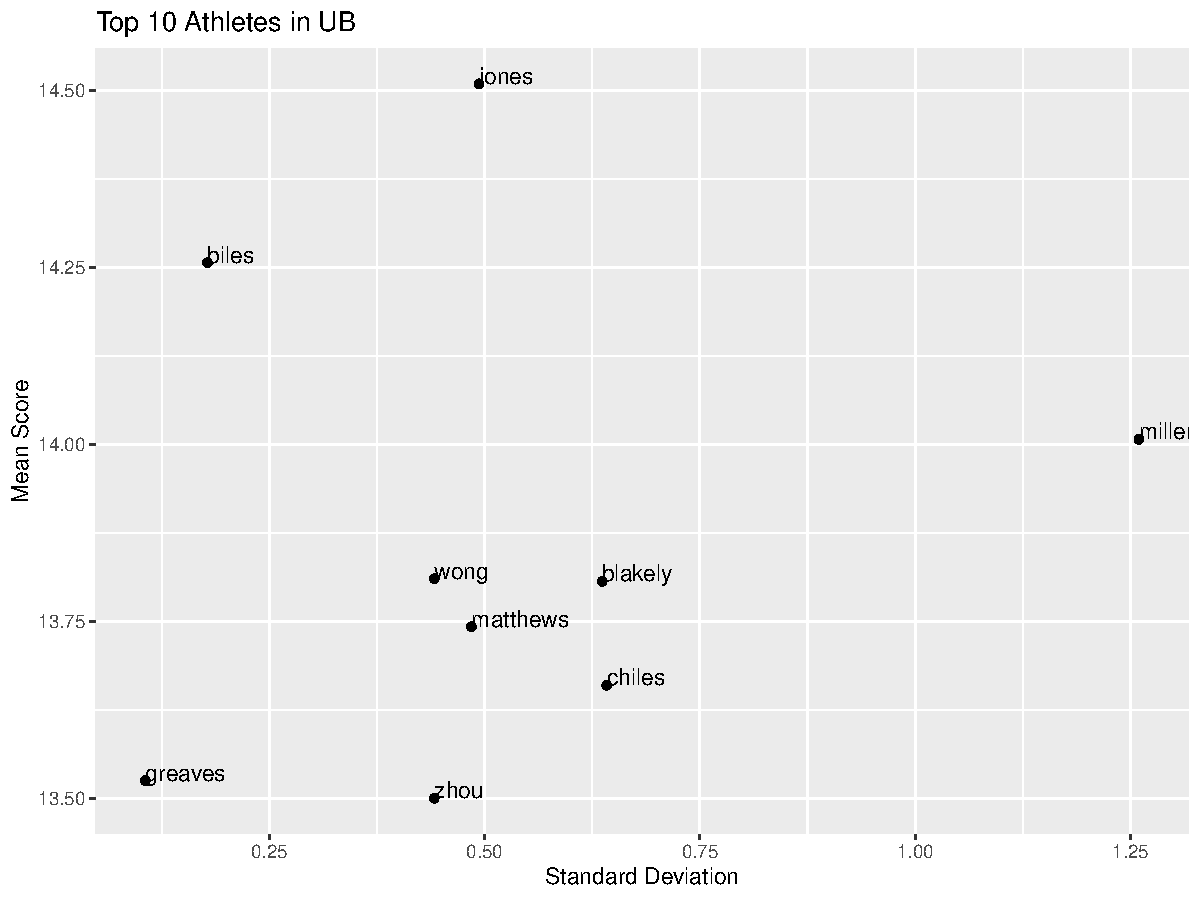
\includegraphics[scale=0.6]{Top10AthletesUB.pdf}
  \caption{Top 10 Candidates for the Olympic Uneven Bar Apparatus}
  \label{fig:UB}
\end{figure}

\begin{figure}[tbp]
  \centering
  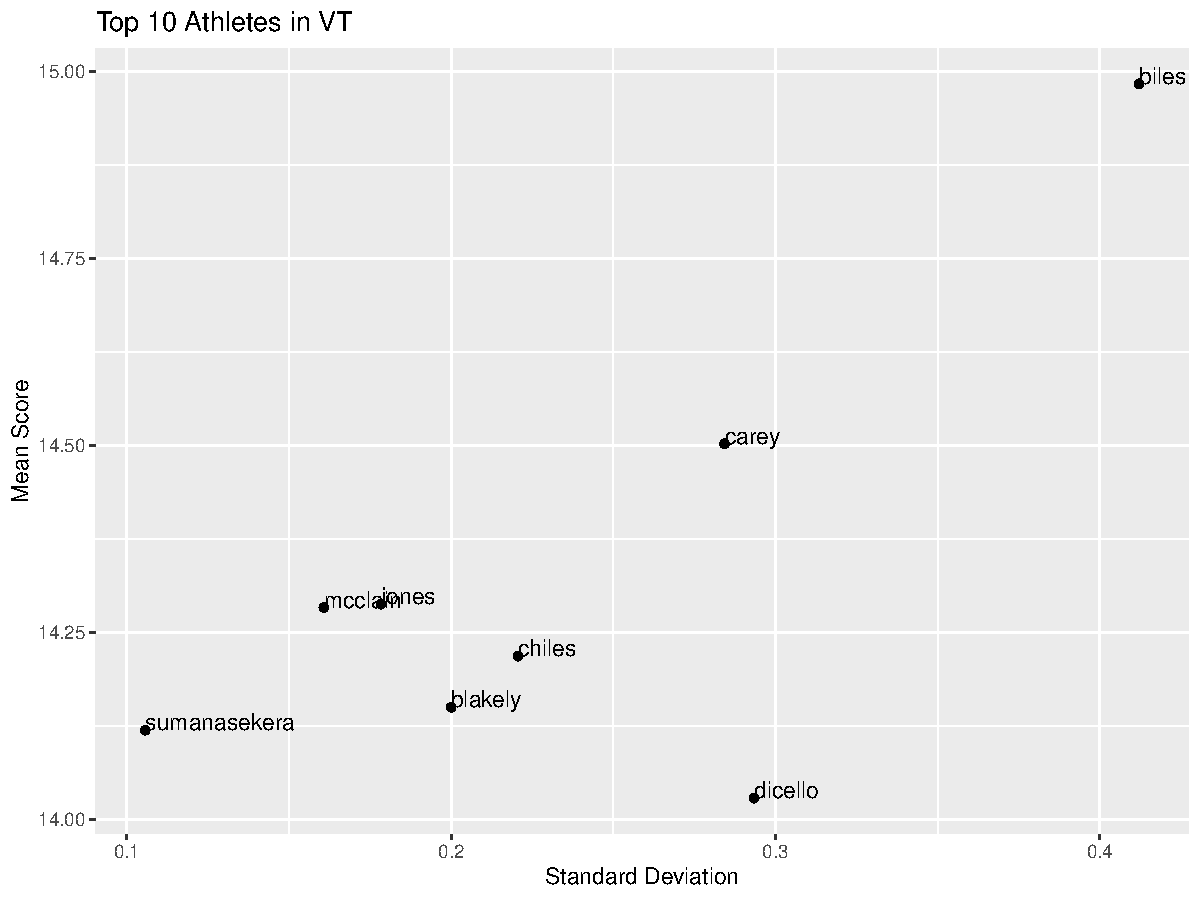
\includegraphics[scale=0.6]{Top10AthletesVT.pdf}
  \caption{Top 10 Candidates for the Olympic Vault Apparatus}
  \label{fig:VT}
\end{figure}

\begin{figure}[tbp]
  \centering
  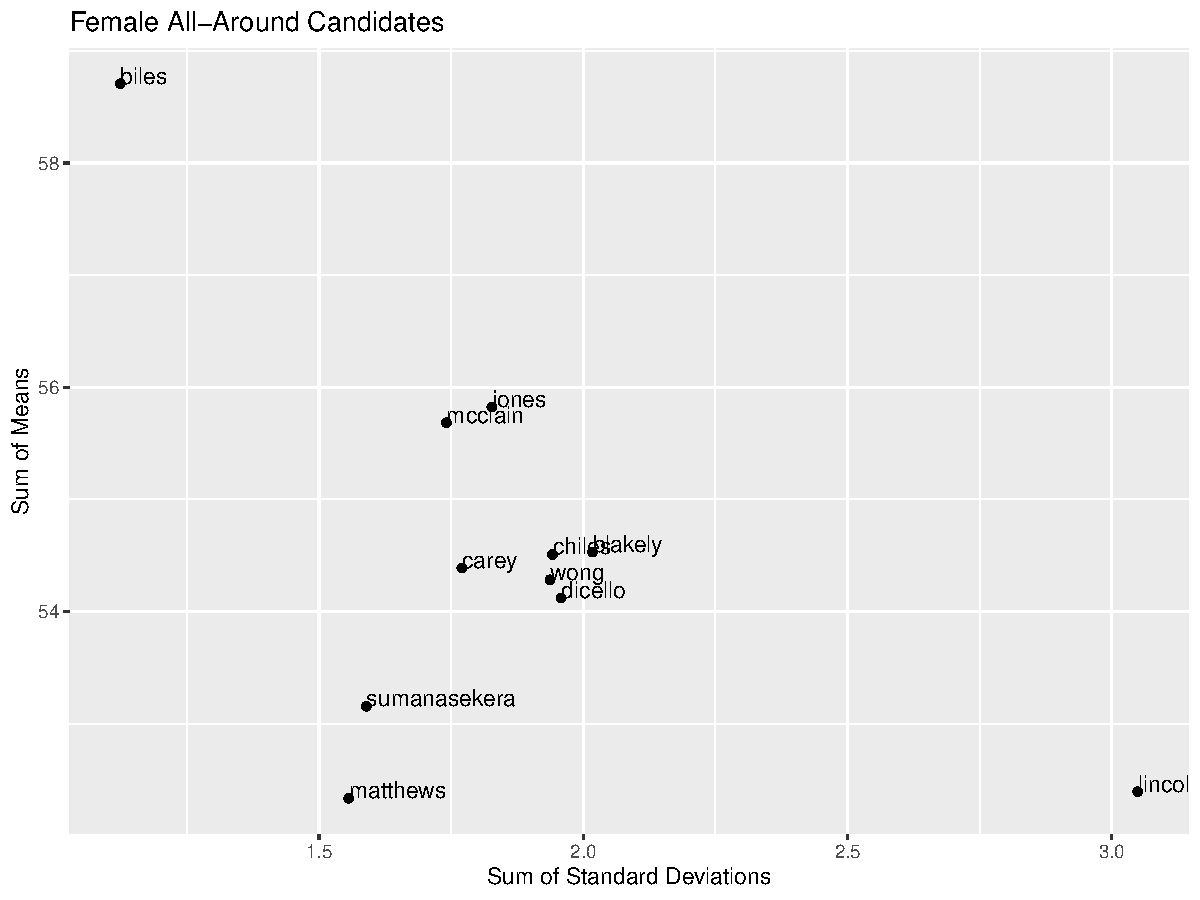
\includegraphics[scale=0.6]{AllAroundCandidates.pdf}
  \caption{The best candidates for the individual all-around medal}
  \label{fig:IAA}
\end{figure}

\begin{figure}[tbp]
  \centering
  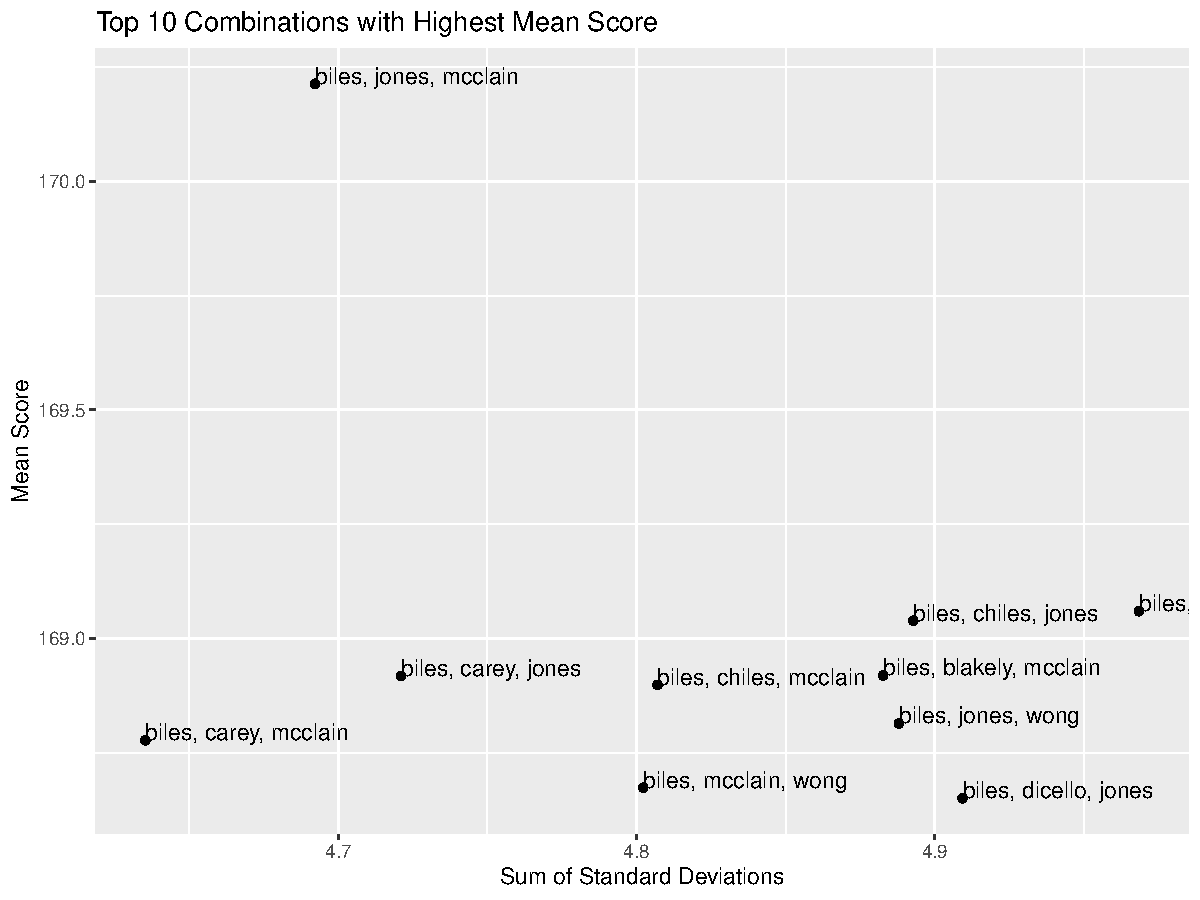
\includegraphics[scale=0.6]{TeamCombinations3.pdf}
  \caption{Top 10 combinations of three candidates for the team all-around medal}
  \label{fig:AA3}
\end{figure}

\begin{figure}[tbp]
  \centering
  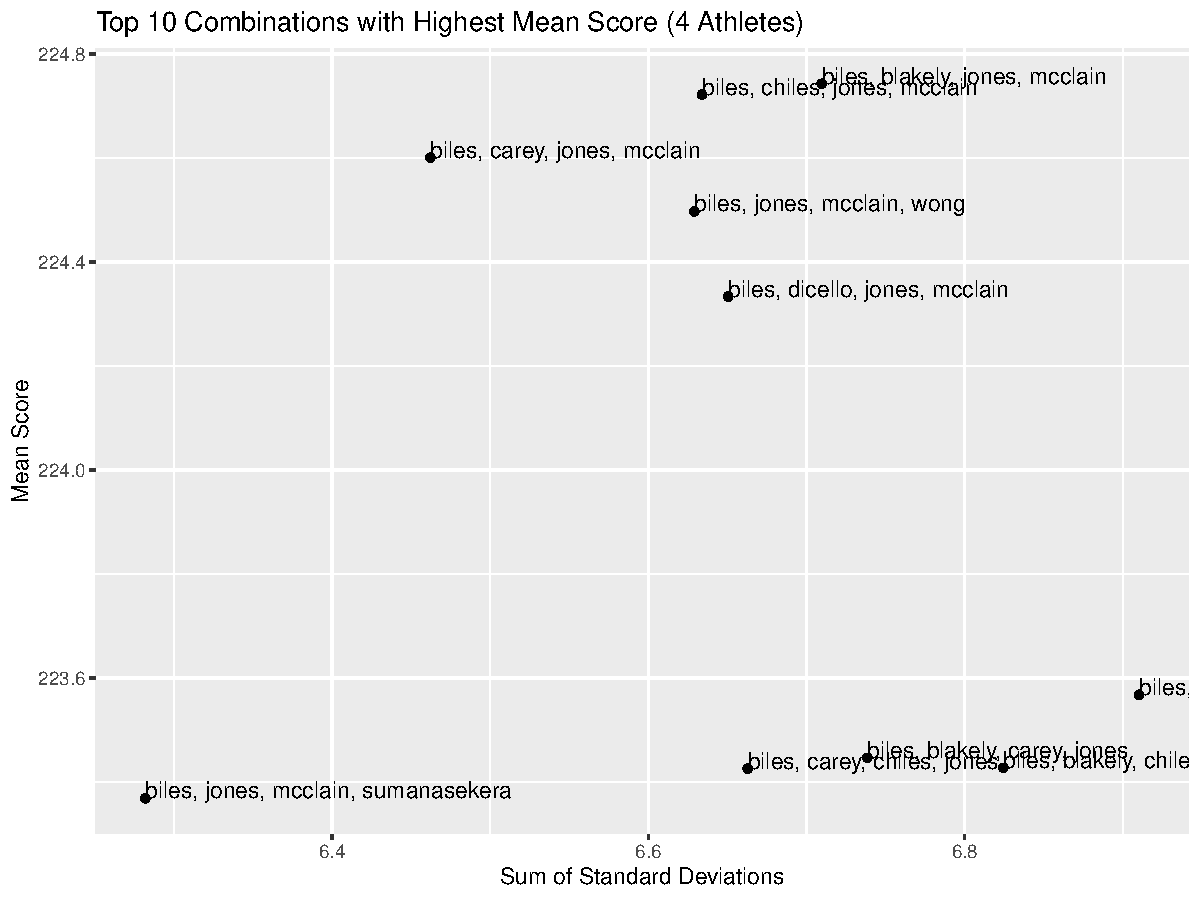
\includegraphics[scale=0.6]{TeamCombinations4.pdf}
  \caption{Top 10 combinations of four candidates for the team all-around medal}
  \label{fig:AA4}
\end{figure}





 



\section{Discussion}
\label{sec:dis}

One of the most challenging parts of this research is that there are no prior studies that have similar
aims to predict olympic success or candidates to model the design and methods off of. Additionally, 
the data challenge source provides so much information that determining which data is most valuable 
can be challenging. Currently, our model is limited as it does not take into account the 
Execution score, Difficulty score, penalty, or importance of specific competitions or rounds over others. 
Furthermore, another limitation of our model is that we generally tried to avoid selecting athletes that
had very few attempts on a particular apparatus even if their few or singular scores were exceptional.

\bibliographystyle{chicago}
\bibliography{citations}

\end{document}